\section{Company profile and reflection on process} \label{company}
As part of AAUs project oriented stay at a company (POSC) the student is expected to deliver a company and project process related description as part of the project documentation. This chapter firstly includes a general description of Vestas as a company including its areas of work its organisational layout and its strategy and culture. Secondly a description of the student's personal payoff from the work at Vestas is included, divided into three parts: Theoretical and practical, work-related and social. Finally suggestions to changes to POSC procedures are listed followed by a reflection on sharing of knowledge between Vestas and AAU.


\subsection{Who is Vestas}
Vestas as a company was officially founded by Hans Smith Hansen and his son Peder Hansen in 1945 under the name VEstjyst STaalteknik A/S which was shortly after shortened to Vestas. In 1979 the first Vestas wind turbine was built with a 10 metre rotor and a 30 kW capacity and in 1995 Vestas built its first offshore wind turbine. As of December 2022 Vestas Wind Systems A/S is the worlds single largest manufacturer of wind turbines in the world with over 29000 employees. Vestas' headquarters is situated in Aarhus, Denmark and houses more than 400 employees. Vestas has currently installed over 160 GW worth of wind turbines in 88 countries with over 8 GW installed offshore.

\smallskip
In contrast to other great turbine manufacturers such as Siemens Games, Vestas handles almost all parts of R\&D, project planning, production, construction, maintenance, support and sales. Vestas both develops and produces its own generators, converters, gearboxes, drivetrains and so forth. Vestas' value chain consists of five steps:
\begin{enumerate}
	\item Research \& development
	\item Project planning \& design
	\item Procurement \& manufacturing
	\item Construction \& installation
	\item Operation \& maintenance
\end{enumerate}

\subsubsection{Organisational layout}

A detailed organisational layout is hard to capture in one diagram because of Vestas' sheer size. In \cref{fig:vestas_organ_layout_1} Vestas' high-level organisational layout is seen. From top down it is observed that both staff functions and executive management reports to the group president and CEO. Executive management across all the areas of work (sales, finance, service e.g.) covers all five regions that Vestas is operating in.
\begin{figure}[ht]
	\centering
	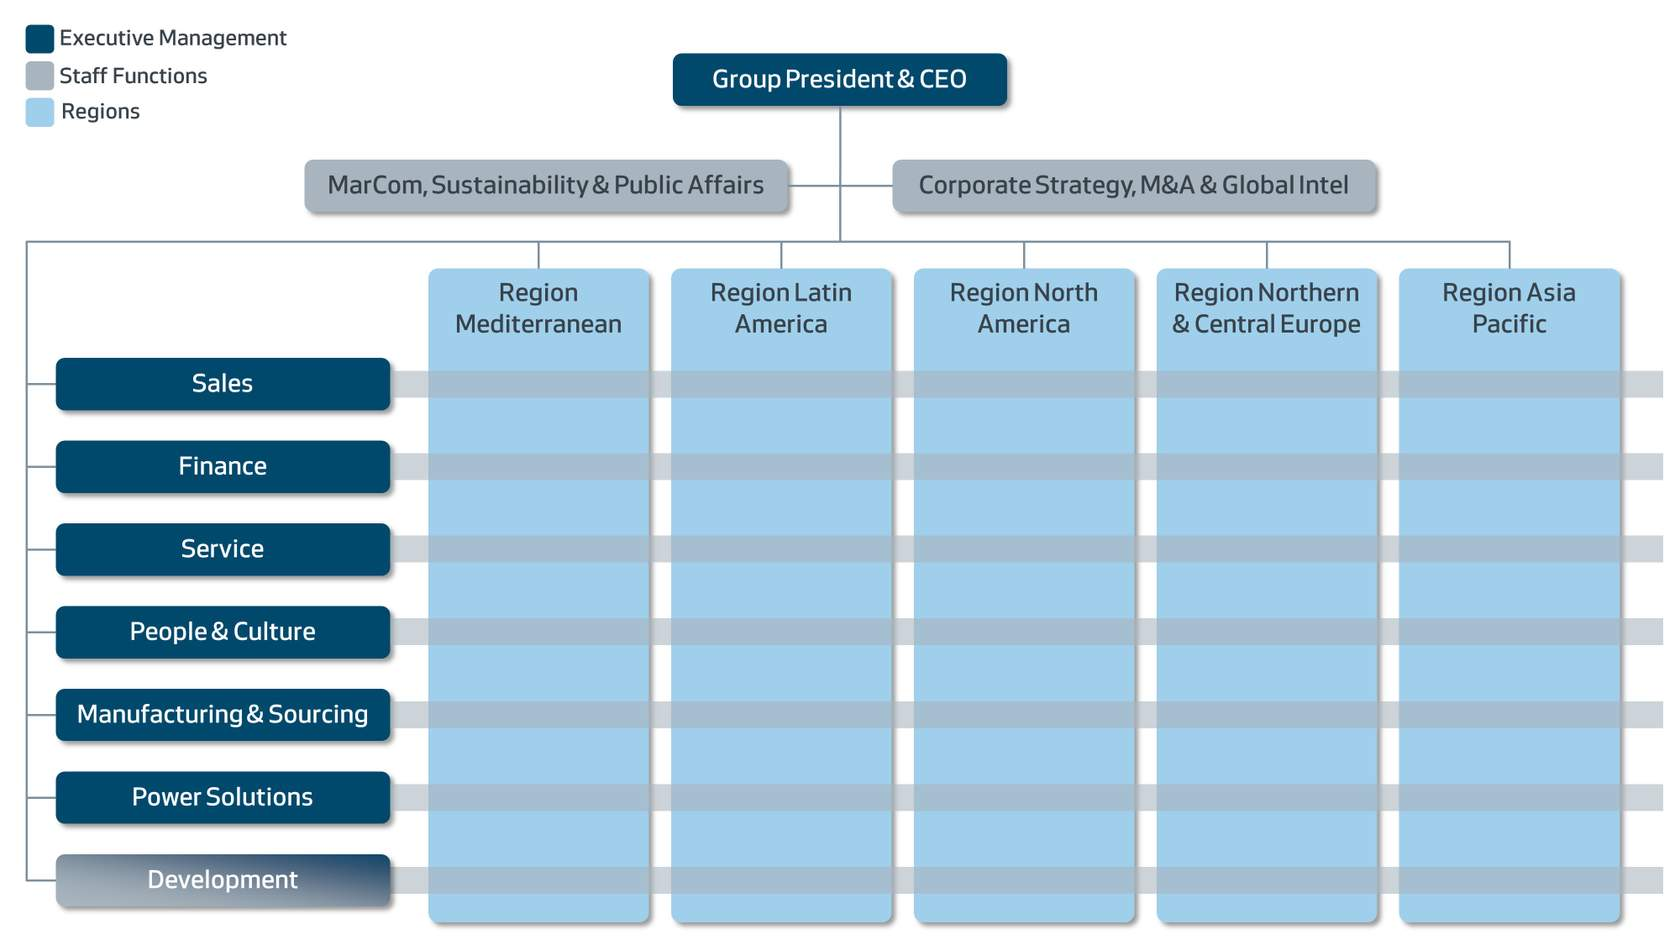
\includegraphics[width=0.8\linewidth]{Graphics/vestasOrganisationalLayout1.jpg}
	\caption{Vestas high-level organisational layout}
	\label{fig:vestas_organ_layout_1}
\end{figure}

\newpage
\subsubsection{Strategy and culture}
Vestas' corporate strategy is largely encapsulated in the Vestas \textit{strategy house} shown in \cref{fig:vestas_strategy_house}. It outlines a top-down strategy in becoming what Vestas calls the \textit{Global leader in sustainable energy solutions}. From top to bottom it shows the
\begin{itemize}
	\item Long term vision
	\item Mid-term objectives
	\item Mid-term priorities and foundation
	\item Core values
\end{itemize}
It also Vestas' intent in being a market leader in revenue by: Growing faster than the market, achieving a EBIT (Earnings Before Interest and Taxes) margin of 10 percent in 2025, having a positive cash flow every year and achieving a Return on Capital Employed (ROCE) of minimum 20 percent. 

\begin{figure}[ht]
	\centering
	\includegraphics[width=0.85\linewidth]{Graphics/vestasStrategyHouse.png}
	\caption{The Vestas \textit{strategy house} which visualizes the hierarchal plan of how Vestas intends to articulate the vision of becoming the \textit{global lead in sustainable energy solutions}}
	\label{fig:vestas_strategy_house}
\end{figure}

\noindent A part of Vestas' foundation for achieving its mid-term strategic priorities is its six \textbf{must-win battles}:
\begin{enumerate}
	\item \textbf{Offshore}: To create the foundation for a global offshore wind leadership in 2025.
	\item \textbf{Sustainability}: To achieve carbon neutrality by 2030 – without using carbon offsets. Reduce CO2-emissions by 55 percent by 2025 across direct operations and over supplier network with 45 percent per MWh delivered to the market by 2030.
	\item \textbf{Quality}: To meet customer expectations and prevent issues from happening by striving to contain and solve them at the root cause, instead of passing them on in the value chain.
	\item \textbf{Modulation}: It combines customisation and standardisation, to make it possible for to serve broad market requirements at competitive costs.
	\item \textbf{Talent \& Leadership}: To become employer of choice in the sustainable energy industry, to attract, develop, and retain the best talents.
	\item \textbf{LEAP}: A quality of service model which is globally aligned and standardised to ensure greater profits while maintaining high service quality.
\end{enumerate}

\medskip
\noindent As part of the onboarding at Vestas a series of learning objectives must be completed. These learning objectives are meant to ensure that every employee is introduced to the strategy and culture of the company. Part of the material introduces the employee to the \textbf{four key values} at Vestas which largely encapsules the culture at Vestas. They are: 
\begin{itemize}
	\item Accountability
	\item Collaboration
	\item Passion
	\item Simplicity
\end{itemize}
While not inherently obvious these four values encapsulates a large and perhaps overwhelming range of ideologies and goals. Among other things \textbf{accountability} means acknowledging personal and interpersonal responsibilities, understanding what's best for all of Vestas and speaking up. \textbf{Simplicity} stands for following the Vestas \textit{Code of Conduct} which is centred heavily on employee safety. It also stands for \textit{clarity of intent} which is meant to ensure that goals, outcomes and objectives are communicated as clearly as possible. \textbf{Collaboration} stands for \textit{integrity and respect} hereunder leading by example as well as \textit{transparency} meaning communicating and engaging with clarity and lastly \textit{inclusion} in the form of diversity. \textbf{Passion} stands for employee motivation in following a shared purpose and motivation for seeking greater understanding and knowledge.



\subsection{Personal payoff from stay at Vestas}
My payoff from my project oriented stay at Vestas split into three main parts: The theoretical/practical payoff, the work-related payoff and the social payoff.


\subsubsection{Theoretical and practical}
Almost all of the theoretical knowledge i have gained throughout my work on the project at Vestas is documented in this report. This subsection will attempt to summarise this knowledge in a manageable form.

\smallskip
Before i started my work i had limited knowledge on wind turbines although i knew the very general layout of WT components and the different turbine configuration types. I also understood the basic WT function and operation with regards to wind conversion to electrical energy in the generator and the subsequent delivery to the grid through the converter. All of my knowledge was although surface level.

To be able to work with the floating problem i had to build a firm foundation of understanding of WTs and WT control on a structural/loads-related level. A list of theoretical gains include but are not limited to knowledge on:
\begin{itemize}
	\item How to model the processes that relate to the energy transfer from the wind to the forces and torques experienced by the turbine rotor.
	\item How a WT controller can work by controlling the turbine based on different operating regions that relate to the wind speed namely PLC and FLC.
	\item How the classical PLC and FLC controllers are set up and what defines the classical operating regions in PLC and FLC.
	\item What periodic disturbances and exciting forces to be aware of with regards to WT control and disturbance rejection.
	\item What causes the negative dampening problem present on FOWTs and how to deal with it.
	\item How to make a simple control-oriented model of a WT in an operating point that captures problem-relevant dynamics while leaving out irrelevant dynamics.
	\item How to make an LQI controller which minimizes system state deviations from an operating point (OP) which contains a reference which is constant.
	\item How the LQI controller might move the closed system poles when changing the $ Q $ and $ R $ weights in a manner which is not obvious or in line with initial hypothesis.
	\item How to use Bryson's Rule to make good initial guesses and tuning LQI $ Q $ and $ R $ matrix weights to get good performance.
	\item How to use simulation tools such as Vestas' VTS to simulate wind turbine loads to both understand turbine behaviour and to tune WT controllers.
\end{itemize}

On a practical level i have learned:
\begin{enumerate}
	\item That employing more theoretical control solutions in the industry can be a very complicated process which can be hard to prove to be economically og practically feasible. 
	\item That simpler control solutions such as PI controllers can be employed with great success in even very complicated non-linear systems such as wind turbines.
	\item LaC tools ..... NEEDS MORE
\end{enumerate}

\subsubsection{Work-related}
What is meant by work-related payoff is: What experience or insight has been gained by being at and working at Vestas in contrast to studying at and being at AAU. Doing work at a company is under normal circumstances different than at a university. There are for an example usually expectations from co-workers or a boss which will expect an output which in some sense creates value for the company or other co-workers. Thus besides perhaps the interest in theoretical knowledge there is further motivation for having good performance. This is unlike work at a university where the sole motivation for putting in work is to gain knowledge, live up to the expectations of project team members and perhaps to pass the exams. In a "\textit{normal}" internship the intern takes on tasks which are present and relevant in the company at the time of the internship. This is different from AAUs POSC because the POSC includes a predefined project proposal which is followed throughout the whole semester. One will therefore come to the conclusion that the POSC work is much like any other project done at AAU. The only major difference is that the project work is done at a company and that you are alone about and can only discuss with co-workers and your POSC supervisor. You are not necessarily participating in the daily project matters and meetings which happen at the company because they are most likely irrelevant to your pre-defined project work.

Therefore I can conclude that on a work-related level i have almost not learned anything i did not already know. Something worthy of mention might be that i have gotten a small insight into how specifically the LaC department runs scrum as a project management tool. This is also at a very surface level, since it has never been made relevant for me. From observing the work environment around me I have furthermore learned that meetings and project planning can make out a huge part of the daily work of an engineer. It is i great contrast to the project work at the university where the way majority of the time is spent working on the technical parts of the project.

\subsubsection{Socially}
I have most days been doing my project work at the Vestas LaC department office. This has given me the opportunity to talk with and socialize with most of the relevant co-workers i have in LaC in Denmark. I have also had the opportunity to ask for help and discuss my project-relevant problems with co-workers when they were not very busy with other matters - which they usually are. But besides the annual Christmas party and some birthday celebrations with cake here and there i have not been invited to many social activities - inside or outside of work. But i am still slightly satisfied with the social outcome of my time at Vestas. Given that my project has never been relevant to anyone but my \textit{buddy} assigned to help me at Vestas I could hardly expect to form deeper friendships with co-workers. This requires time and ideally that i do some work in corporation with my other co-workers. In my experience the people working at Vestas are polite, friendly and social while maintaining professionalism. The social environment seems great and would i get the chance to work in LaC I would expect to have a good time.

\subsection{Suggestions on changes to the curriculum and procedures}
I would suggest that the POSC did not suggest that all work to be done throughout the project is predefined but also leaves room or even suggests that the intern takes on company/department relevant tasks which would engage the student more in the daily work done in the company. As it stands POSC ends up being no different than a less anxiety inducing masters degree done at a company. If the goal was to have the student be more engaged in the daily work at the company as to actually get a feeling of how it is to work at a company then the POSC guidelines should attempt to ensure that the student is assigned to tasks which are carried out with co-workers. This semester we were three students doing an internship at Vestas and the story is the same for all of us. Our work is almost completely cut off from the work done by co-workers. This problem might be more specific to Vestas than it is to POSC in general but i can only speak from my own experience and the experience of my peers here at Vestas.


\subsection{Reflection on sharing of knowledge between Vestas and AAU}
Vestas will of course have gained some knowledge through the work that I have done on the project. But ss it stands there has been no knowledge sharing between Vestas and AAU through my project work except the knowledge that my AAU supervisor might have gained by supervising me - and of course perhaps the knowledge that AAU can gain from the report I am writing. Other than that i can not think of any channel which should have resulted in knowledge sharing between Vestas and AAU. The meetings which have included both Vestas and AAU have been directly aimed at helping me progress with my project work and my report. This might be exactly what is meant by sharing of knowledge but i do now know.
